\chapter[Classification]{Classification} 
\label{chapter:text}
\begin{center}
{\Large\textit{\ldots }}
\end{center}
\vspace{0.2in}

\section{A Quick Introduction}

    Classification is one of the fundamental problems of machine learning and data science in general. Whether you are trying to create a `spam' filter, trying to figure out which patience are most likely to be hospitalized in the coming year, or trying to see tell whether a particular image appears in a photograph, it is all too likely that you will spend a significant percentage of your time working on such problems. There are two basic types of classification: the binary (or two-class) and the multi-class problem. In this chapter we will explore some of the basic solutions constructs and evaluations thereof.

    
\section{Naive Bayes}
\label{NB}


The \T{Naive Bayes classifier} is probably the most fundamental and widely used methods in industry today. It is simple, fast, easily updated and, despite it's many theoretical and even technical pitfalls, quite effective in practice. Many a time will the real-life limitation of an industry solution lead you to drop a more sophisticated approach where the accuracy gains do not justify the time and resources for this relatively trivial approach. 


Lets take a sample problem. Suppose you built a news aggregation site which pulls in article publication data from a myriad of sources. In order to organize this information you would like to be able to classify the incoming articles automatically and place the corresponding links in the appropriate section on your site. Say for simplicity, you have three classes of articles, labelled \T{leisure, sports} and \T{politics}. 

If you had no information at all about the articles themselves, you would be temped to simply assign the most common label. For example, if on an initial scan you realized you had $20\%$ \T{leisure}, $30\%$ \T{sport} and  $50\%$ \T{politics} your best bet would be to assign \T{politics} to article and then regularly redo the count. However, suppose you knew that the word "sports" appeared in $2\%$ of the \T{leisure}, $95\%$ \T{sports} and  $3\%$ \T{politics} articles you'd likely want to shift the initial, or prior, distribution of labels by this new information. With a few seconds of thoughts you'd probably write down the following:


\begin{align*}
    P(label|hasword(``sport")) = P(hasword(``sport")|label)P(label)
\end{align*}
and
\begin{align*}
    P(hasword(``sport")|label) = \frac{P(hasword(``sport"),label)}{P(label)} \\ = \frac{count(hasword(``sport"), label)}{count(label)} 
\end{align*}

i.e. the new article would receive a classification score of $.2*.02$ for \T{leisure}, $.3*.95$ for \T{sport} and $.5*.03$ for \T{politics}, which is more sensible given the new information. If you continued to explore the language, extract tags and feature as in the text processing chapter you would assume to increase the accuracy of your classifier. 


With the intuition above we have practically arrived at the construction of a \T{naive Bayes classifier}, so lets write down the details. 

Given a set of labels $L = \{l_1, \dots, l_N\}$ and set a features $\mathcal{F}$ we can calculate the probability that a given article has label $l_i$ with

\begin{align*}
    P(l_i|\mathcal{F}) \propto P(\mathcal{F}|l_i)P(l_i).
\end{align*}

This is, if course, just the max likelihood calculation coming from Bayes theorem, but if add the assumption that the features are \T{conditionally independent} we arrive at our classifier, i.e. 

\begin{align*}
    P(l_i|\mathcal{F}) \propto P(l_i)] \prod_{f \in \mathcal{F}} P(f|l_i),
\end{align*}

with each $P(f|l_i)P(l_i) = \frac{f, l_i)}{count(l_i)}$ as above. The ``naivety''  comes from the fact that most feature are indeed dependent and sometime highly so. 

Hence, the classifier will assign the label $l$ where  

\begin{align*}
    l = \arg \max_{l_i \in L}P(l_i|\mathcal{F}) 
\end{align*}

to an item with a give feature set $\mathcal{F}$.



An astute reader would immediately raise at least three objects to the above setup:

\begin{itemize}

    \item Over counting. Imagine that you have an extreme case, where two variables are not just dependent but are actually the same feature repeated. Then instead its contribution to the likelihood will for that feature will be double what it should have been.
        
        As another example, suppose in addition to the three labels above you also consider individual sports. You have two features, one of which detects whether or not the article contains number and the other if the article contains the number $0,15,30,40$ (tennis point calls). Whenever you will see an article with $0,15,30,40$ the posterior will be boosted by not only the fact that these specific number are present but also by the feature that detects number at all. This example might seem pathological, but this is essentially what happens when you have dependent features appearing in the \t{naive bayes setup}. 

        
    \item If the training set is not fully representative this could lead to many of the $P(l_i|\mathcal{F})$ being equal to zero. Suppose you have arrive at a situation where a new article, which should have some particular label $l_i$, contains a feature $f$ which never appears with $l_i$ in the training set. Then the corresponding probability count $P(f|l_i)=0$ which forces $P(l_i|\mathcal{F})=0$ no matter what the other counts are telling you. This can lead to misclassification and, frequently, does since it is generally hard to make sure that your training set is truly representative. 

        Consider the example in the situation above where you see an incoming article with the phrase ``boxing match.'' This could refer to a sporting event but can also simply be an simile describing the way the Russian parliament behaves itself. If you have no example of articles labelled \T{politics} containing this phrase, your classifier will make a mistake.

    \item If enough of the probabilities $P(f|l_i)P(l_i)$ are sufficiently small this can lead to \T{floating point underflow}, causing $P(l_i|\mathcal{F})$ to be zero once again.

        Floating point number don't have infinite precision (open up your python shell and type 1e-320 if you want to convince yourself) and, hence, after a certain point these are rounded to zero. In general if you have a large training set, as you should, you will have many instances where the value of  $P(f|l_i)P(l_i)$'s is small; multiplying these will result in \T{underflow}, causing the posterior to be zero. There are ways to handle ushc issues in the python \T{decimal} module, but we will look at some others below. 
        
 
\end{itemize}


\subsection{Smoothing}

Probably the most common solution to the latter two issues above is called \T{arithmetic smoothing}. Here we simply add constant to each likelihood above, i.e. replace with $P(f|l_i)P(l_i)$ with

\begin{align*}
P(f|l_i)P(l_i) + \alpha
\end{align*}

If $\alpha=1$ this is referred to as \T{one-smoothing}, but generally a smaller value such as $.5$ is chosen. 

Another solutions is to transform everything onto the logarithmic scale, i.e. effectively replacing multiplication with addition. We can then write our classifier as 

\begin{align*}
    l = \arg \max_{l_i \in L} \log [P(l_i) \prod_{f \in \mathcal{F}} P(f|l_i)] = 
    \arg \max_{l_i \in L}  [\log P(l_i) + \sum_{f \in \mathcal{F}} \log P(f|l_i)] 
\end{align*}


\vspace{15mm}
\section{Measuring Accuracy}

\subsection{Error metrics and ROC Curves}
\label{classification:subsection:roc}


A classifier either gets something right or wrong. Although looking at various statistical error metrics such as \T{rmse} can be useful for comparing one classifier model, the most natural is to look at predicted vs true positives and negatives, i.e. the ratio of how many times the model got something right vs wrong. There are a few essential terms that come along with the territory: an instance that is positive and is classified as such is counted as a \T{true positive}; if the same positive instance is classified as negative the it called a \T{false negative}. Similar for \T{false positive} and \T{true negative}. For this you naturally arrive at a $2x$ matrix of true and predicted classes called a \T{confusion matrix} or a \T{contingency table}, as you can see below:

\begin{figure}
  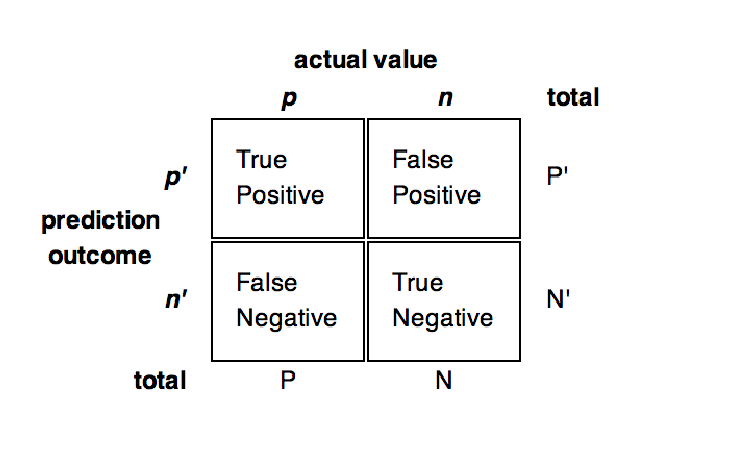
\includegraphics[width=.8\textwidth,height=0.3\textheight]{../images/confMatrix}
  \caption{Predicted vs actual in a 2-class situation}
  \label{class:confMat}
\end{figure}

\newpage

Given the long history and wide application of classifiers there is a plethora of terminology for the key quantities. 

\begin{itemize}
        \item True positive rate (or hit rate, recall, sensitivity)

            
            $$tp\hspace{2mm}rate = \dfrac{Positives\hspace{2mm}correctly\hspace{2mm}classified}{Total\hspace{2mm}positives}$$ 

        \item False positive rate (or false alarm rate)

            
            $$fp\hspace{2mm}rate = \dfrac{Negatives\hspace{2mm}incorrectly\hspace{2mm}classified}{Total\hspace{2mm}negatives}$$ 


         \item Specificity
            
             $$specificity = \dfrac{True\hspace{2mm}cnegatives}{False\hspace{2mm}positives\hspace{2mm}+\hspace{2mm}True\hspace{2mm}negatives} = 1 - fp\hspace{2mm}rate$$

\end{itemize}


             To get a feeling at what these quantities represent, lets just look at a few. \T{sensitivity}, or the \T{true positive rate} is proportion of the actual positives correctly classified as such; and the \T{specificity}, or true negative rate, is the proportion of actual negatives correctly classified as such. So a perfect classifier will be $100\%$ sensitive and $100\%$ specific. You can interpret the other quantities in a similar fashion.
             The reason these quantities can be important, as opposed to another standard model error metric such as \T{RMSE}, is that a model and the associated error never live in a vacuum, i.e. the error should not only give you a metric for model comparison but also convey its accuracy and validity as applied to the situation you are trying to predict or understand. For example, suppose that you are asked to build a classifier whose task it is to predict which amazon user is going to open at least one advertisement email in the next week (for say better email ad targeting). You might find it acceptable to have a model which gives a true positive and true negative rate of $70\%$ because you care equally about sending emails to those who will open and not sending to those who don't. But suppose that next you are asked to build a classifier which is going to predict whether some combination of financial signals should constitute opening a trade position, but you know that the potential loss and gain of any such trade is high. Given that you are likely risk averse you would probably care more that the false negative rate being as low as possible than anything else, i.e. you would be ok with potential missing a good trade but not ok with loosing a large amount.

             Some classification models, such as \T{Naive Bayes}, provide a strict probability for a class given a set of features; otherwise, such as the popular \T{gradient boosting decision tree} classifier, provide a score indicating the level of classification. For example, if you have a two-class problem the output might be on a scale $[a,b]$ where $a$ and $b$ are some numbers close to $0$ and $1$, respectively. Here the classifier simply orders your test cases from those closest to the class $0$ to those closest to the class $1$. Hence, there is no reason to a priori select some threshold such as $.5$ as the cutoff; with every new threshold you will get a new set of classifier error quantities which you can use to understand the general `quality' and robustness of your classifier, as well as an optimal cutoff point. This leads us to \T{Receiver Operator Curves} or \T{ROC}. 

             Given a classifier $\mathcal{C}$, an \T{ROC} take in a threshold value $T$ and returns the tuple (tp rate, tn rate), i.e. 


\begin{align*}
    ROC_{\mathcal{C}}(T) = (fp\hspace{2mm}rate, tn\hspace{2mm}rate), 
\end{align*}


or $ROC_{\mathcal{C}}: [-\inf, \inf] \rightarrow [0,1]\x[0,1]$ which is a curve in the plane. 


There are a couple of points of note here: the point $(0,0)$ indicates that no actual positives have been predicted but no false negatives either, i.e. this point represents the threshold $\inf$ where no $1$'s were predicted; the point $(1,1)$ is the other end of the spectrum, where every point was classified as $1$ resulting in $100\%$ true positive and false positive rate; the point $(0,1)$ represents the perfect classifier, with no points classified as false and no true classification being wrong. In addition, the diagonal represents the random classifier, since we expect it get the same proportion right as it get wrong. Hence, a classifier with an \T{ROC} curve above the diagonal is better than random and below the diagonal is worse than random. 
\begin{figure}
  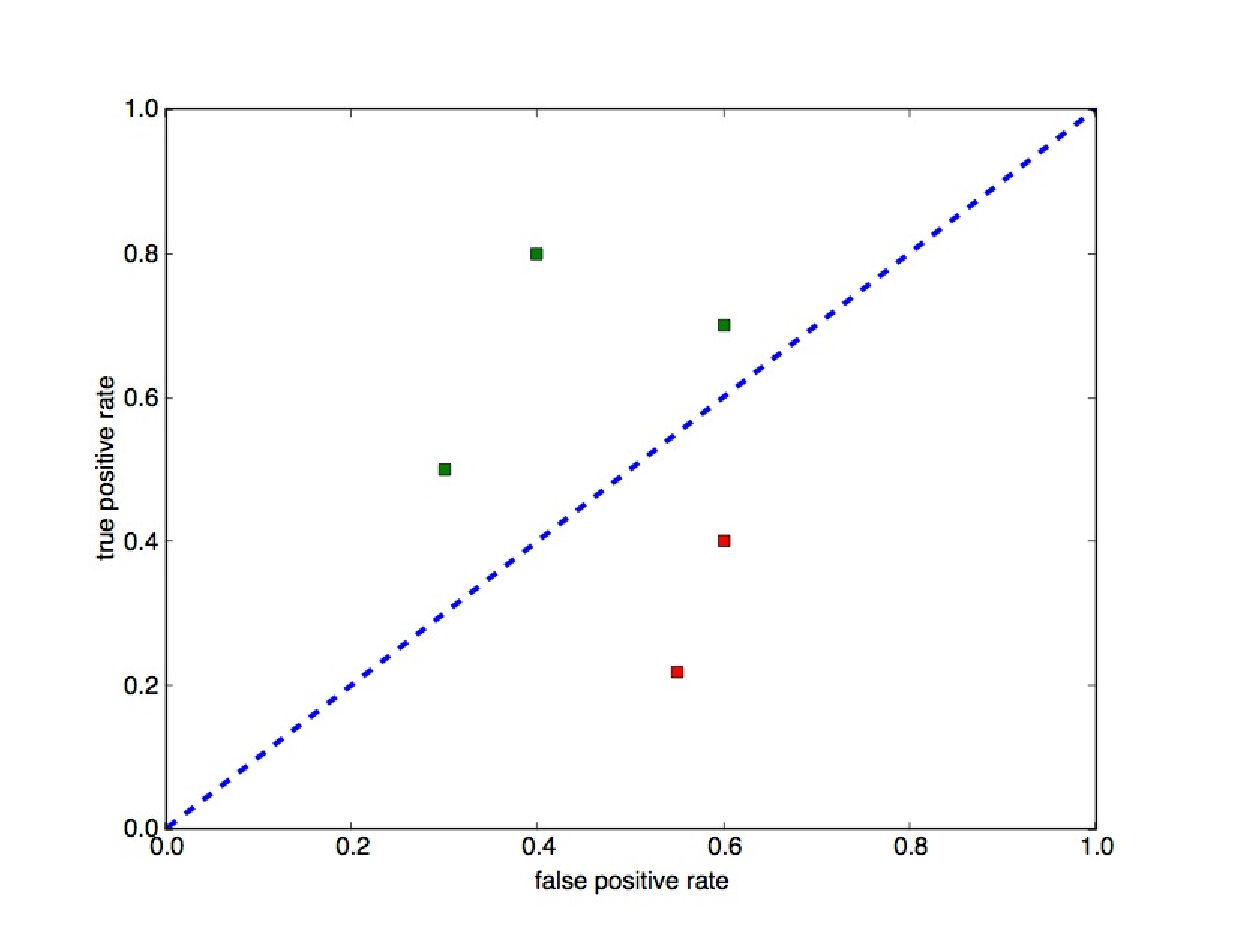
\includegraphics[width=.9\textwidth,height=.45\textheight]{../images/rocRand}
  \caption{The green squares represent classifiers that are better than random and the red squares represent those worse than random}
  %\label{class:confMat}
\end{figure}


By now you can probably guess how to write a simple \T{ROC} algorithm and we take out verbatim from \cite{ROC}. Essentially you order the test cases based on predicted value, from highest to lowest and then start sequentially including the points into the set of positive classifications. With every new point if it is in fact positive you will increase you true positive rate, keeping your false positive rate constant, and if it negative the true positive rate will stay the same while the false positive will increase. Hence, you will either move vertically or horizontally on the plane - lets look at an example below. 

\begin{example}

    Suppose you have a test set of $10$ cases, whose actual class you know, and you classifier outputs the following numbers. The cases are listed below in descending order. 


\begin{center}
    \begin{tabular}{c|c|c}
        \hline
        case & Class(case) & actual \\ \hline
        1 & .97 & True \\ \hline 
        2 & .93 & True \\ \hline 
        3 & .87 & False \\ \hline 
        4 & .70 & False \\ \hline 
        5 & .65 & True \\ \hline 
        6 & .58 & False \\ \hline 
        7 & .43 & True \\ \hline 
        8 & .33 & False \\ \hline 
        9 & .21 & True \\ \hline 
        10 & .05 & False \\ \hline         
    \end{tabular}
\end{center}


\begin{figure}
  \label{class:rocEx}  
  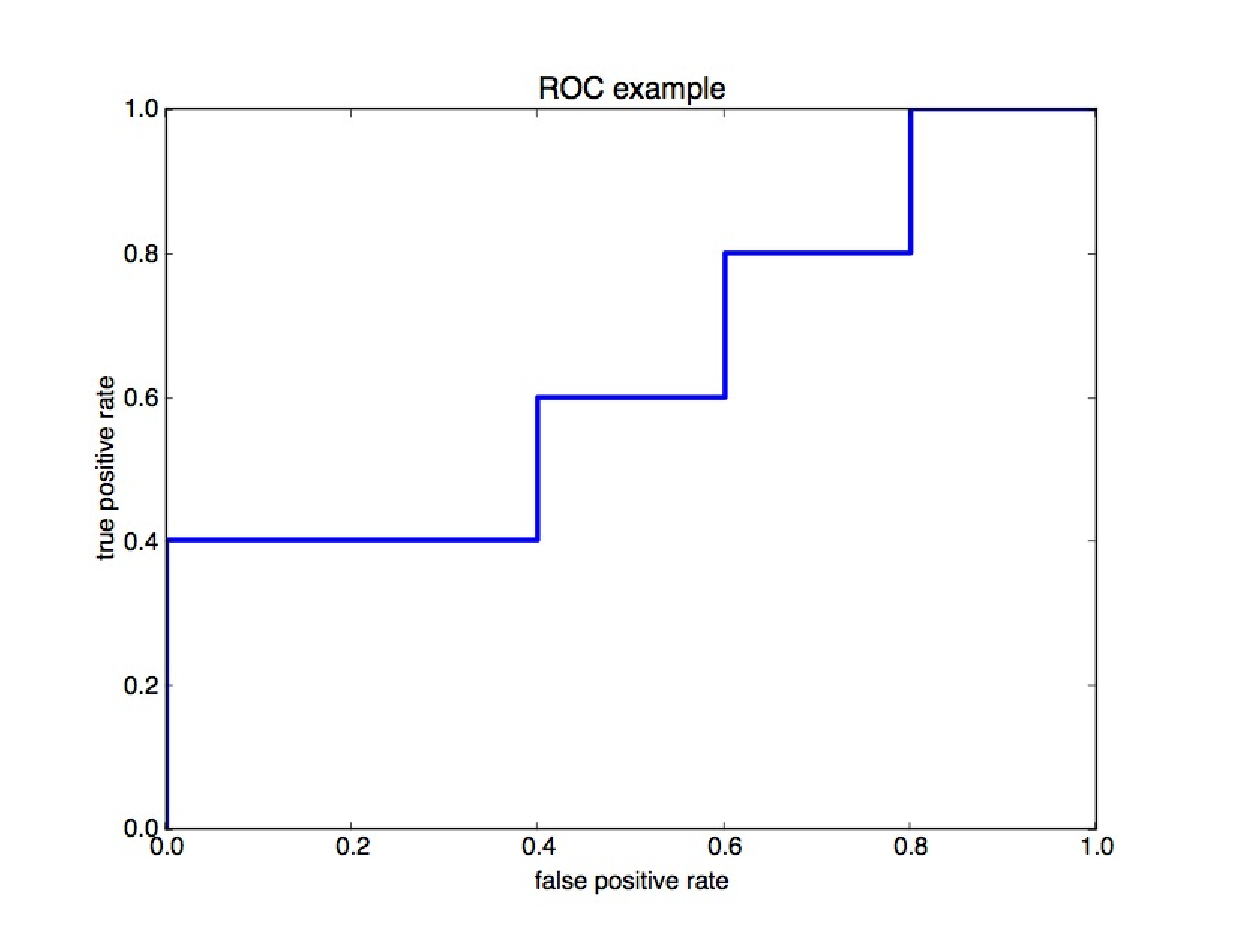
\includegraphics[width=\textwidth,height=.45\textheight]{../images/rocEx}
  \caption{Our example \cal{ROC}}
\end{figure}

With the first threshold, $-\inf$, you classify no cases as true and, hence, have no true or false positives, i.e. the first point on $\mathcal{ROC}$ is $(0,0)$. With the second threshold you will classify the case $1$ as true; since this is correct your true positive rate will now be $\frac{1}{5}$, since there are $5$ positives int the test set, and your false positive rate will be $0$. With the third threshold you will classify cases $1$ and $2$ as true, leading to $\frac{2}{5}$ tp rate and $0$ tn rate, etc In figure \ref{class:rocEx} you can see the $\mathcal{ROC}$ plotted for this example. 
\end{example}



Below is an efficient $\mathcal{ROC}$ algorithm copied verbatim from \cite{ROC}. 

Inputs: $L$, the set of test examples; $f(i)$, the probabilistic classifier's estimate that example $i$ is positive; $P$ and $N$, the
number of positive and negative examples.


Outputs: $R$, a list of $\mathcal{ROC}$ points increasing by fp rate.


Require: $P > 0$ and $N > 0$


\begin{algorithmic}
    \State $L_{sorted} \leftarrow L$ 
    \State $FP \leftarrow TP \leftarrow 0$
    \State $R \leftarrow <>$
    \State $f_{prev} \leftarrow -\inf$
    \While{$i \leq |L_{sorted}|$} 
 \If{$f(i) \neq f_{prev}$} 
 \State push$(\frac{FP}{N}, \frac{TP}{P})$ onto $R$
 \State $f_{prev} \leftarrow f_i$
   \EndIf
   \If{$L_{sorted}[i]$ is a positive example}
      \State $TP \leftarrow TP + 1$
      \Else /* $i$ is a negative example*/
      \State $FP \leftarrow FP+1$
   \EndIf
   \State $i \leftarrow i+1$
\EndWhile
\State push$(\frac{FP}{N}, \frac{TP}{P})$ onto $R$ /* This is (1,1) */
\end{algorithmic}


\section{Other classifiers}


\subsection{Decision Trees}


Decision trees form a fundamental part of the classification, as well as the regression, toolbox. They are conceptually simple and in many instances very effective. 
There are a few basic terms necessary before we dive in: a \T{decision node}, or simply \T{node}, is a place-holder in the tree which signifies a decision being made (in the case of a binary feature, the split will be on whether an item from the data set satisfies the feature conditions); the \T{leaves} of a decision node are class labels. 

The basic algorithm is the following:

\begin{enumerate}

    \item Begin with a decision stump. This is simply a collection of trees consisting of a single node, one for each feature. 
    \item Pick the best one, i.e. given some sort of accuracy measure (\T{splitting objective}) select the single node tree which is the most accurate. 
    \item Check the accuracy of each leaf by evaluating the assigned classification on the associated subset of data. If the accuracy is not sufficiently high, i.e. does not satisfy some pre-defined criteria, continue building the tree as in step 1  utilizing the unused features on the associated subset of data.
\end{enumerate}

Geometrically, decision trees tile your data space with hyper-rectangles, where each rectangle is assigned a class label. There are a number of advantages:

\begin{itemize}

    \item Decision trees are simple and easy to interpret.
    \item They require comparatively little data cleaning (can deal well with continuous, or categorical variables).
    \item Evaluation of a data point is fast, $\log(n)$ where $n$ is the number of leaves.
    \item Can handle mixed-type data.
        
\end{itemize}


The main drawbacks are the following:

\begin{itemize}

    \item Decision trees can easily become complex and lead to over-fitting. One way to deal with this problem is to \T{prune}, by either setting the minimum number of samples for a given node to split (if the min samples is high, the tree is forced to make a decision early, fitting the data less) or by setting the \T{max depth}, limiting the entire size of the tree.
    \item The prediction accuracy can become unstable with small perturbations of the data, i.e. a small ``shift'' can lead to data points falling into the wrong classes. \T{Ensembling} many trees, which we will look at below, can help mitigate this problem.
    \item Finding an optimal tree is NP-complete. Note, that the algorithm described above does not guarantee that a globally optimal tree is found, since it simply makes the best decision at any given node excluding the possibility that say a less than optimal decision locally might lead to a better overall classifier. 
\end{itemize}



For more information about decision trees, see Python's \T{scikit-learn} library. 


        

\subsection{Random Forest}

\T{Random Forest} is a popular ensemble method, whose creation is attributed to Leo Brieman, Adele Culer, Tin Kam Ho, as well as others. The method aims to utilize the flexibility of a single decision tree, while mitigating the drawbacks mentioned above by spreading them out over an entire collection. Random forest, like ensembles in general, can be thought of as a framework more than a specific model. The essential pieces are the following:

\begin{itemize}
    \item The shape of each decision tree, i.e. is the threshold for a single decision a liner, quadratic, or other function.
    \item The type of predictor to use at each leaf; for example, a histogram of constant predictor.
    \item The splitting objective to optimize each node; for example, error rate, information gain, etc.
    \item Some random method which will specify each tree. 
\end{itemize}

For the sake of concreteness, and to set up the some of the technicalities which will help us understand why random forests make sense as an classification approach, lets look at Brieman's original definition and algorithm.
            
\vspace{.3in}

\begin{definition} (Brieman) A \T{random forest} is a classifier consisting of a collection $\{h(X, \theta_k)\}_{k=1, \dots}$ where $\{\theta_k\}$ are independently distributed random vectors and each tree counts a unit vote for the most popular class at input $\overline{x}$.
\end{definition}




For each tree, Brieman specified to do the following:

\begin{enumerate}
    \item Let $N$ be the number of training cases and $M$ the number of features in the classifier. 
    \item Let $m$ be the number of input features that are used to determine the decisions at the tree nodes; $m<<M$. 
    \item Choose a training set of size $n \leq N$, with replacement, and use its complement as a test set. This is know as a \T{bootstrap sample}.
    \item Choose $m$ features which will be used for decisions in the given tree and calculate the best split on those features and training set. 
    \item Let each tree be fully grown, i.e. no pruning. 
\end{enumerate}

The result is a collection of trees $T_{1}, \dots , T_{K}$ where given a input $\overline(x)$ a class can be assigned by taking the mode vote over all the $T_{i}$'s. Note, this was Brieman's original approach; for regression trees, or if you are interested in knowing the strength of a given classification, an average or some other weighted sum can be taken over the outputs of the $T_{i}$'s.


Although $m$ can be determined experimentally, many packages use $\sqrt{M}$ or $log_2(M)$ as default values. 



\subsection{Out-of-bag classification}


Given a collection of \T{bootstrap samples} $T_{1}, \dots, T_{k}$ from a training set $T$, as well as pair $\overline(x), y \in T$, you can use the classifiers trained on samples $T_i$ where  $\overline(x), y \notin T_i$ for measuring the prediction accuracy. For example, suppose you have samples $T_{1}, T_{2}, T_{3}$, and respective trained classifiers $h_{1}, h_{2}$ and $h_{3}$, as well as a pair  $\overline(x), y \in T_{1}$ but  $\overline(x), y \notin T_i$ and  $\overline(x), y \notin T_2$. You can predict the accuracy of your ensemble classifier from evaluating $h_{2}(\overline(x))$ and $h_{3}(\overline(x))$, against the true value $y$. 



This is called an \T{out-of-bag estimate}, or \T{classification}, and empirical evidence has shown that in practice the setup up is as good as using a train/test set of equal size. If your training set is small and you are worried about leaving some part of it out during the model build, this can be a good approach. If your training set is very large, and you are worried about computation time, you can use smaller \T{bootstrap} samples to build a collection of classifiers in less time and ensemble these together. Since the individual classifiers are independent you can make parallelize the whole process making it highly scalable, which can be very useful if you envision having to retrain your models in the same way but on ever growing data sets.  



\subsection{Maximum Entropy}


There are a number of different criteria which you can use to split a decision tree node, and one very popular which we will look at now is called \T{maximum entropy}. You can think of \T{entropy} as the information content, the measure of uncertainty, or randomness of a random variable. 

The \T{entropy} of a random variable $X$ is define as 

\begin{align*}
    H(X) = - \sum_{i \in Class} P(X=i)log_{2}P(x=i)
\end{align*}

where the sum is over all the classes the random variable can output. \ref{class:entropy} shows a plot of what the function would look like for a two-class variable. 

\begin{figure}
  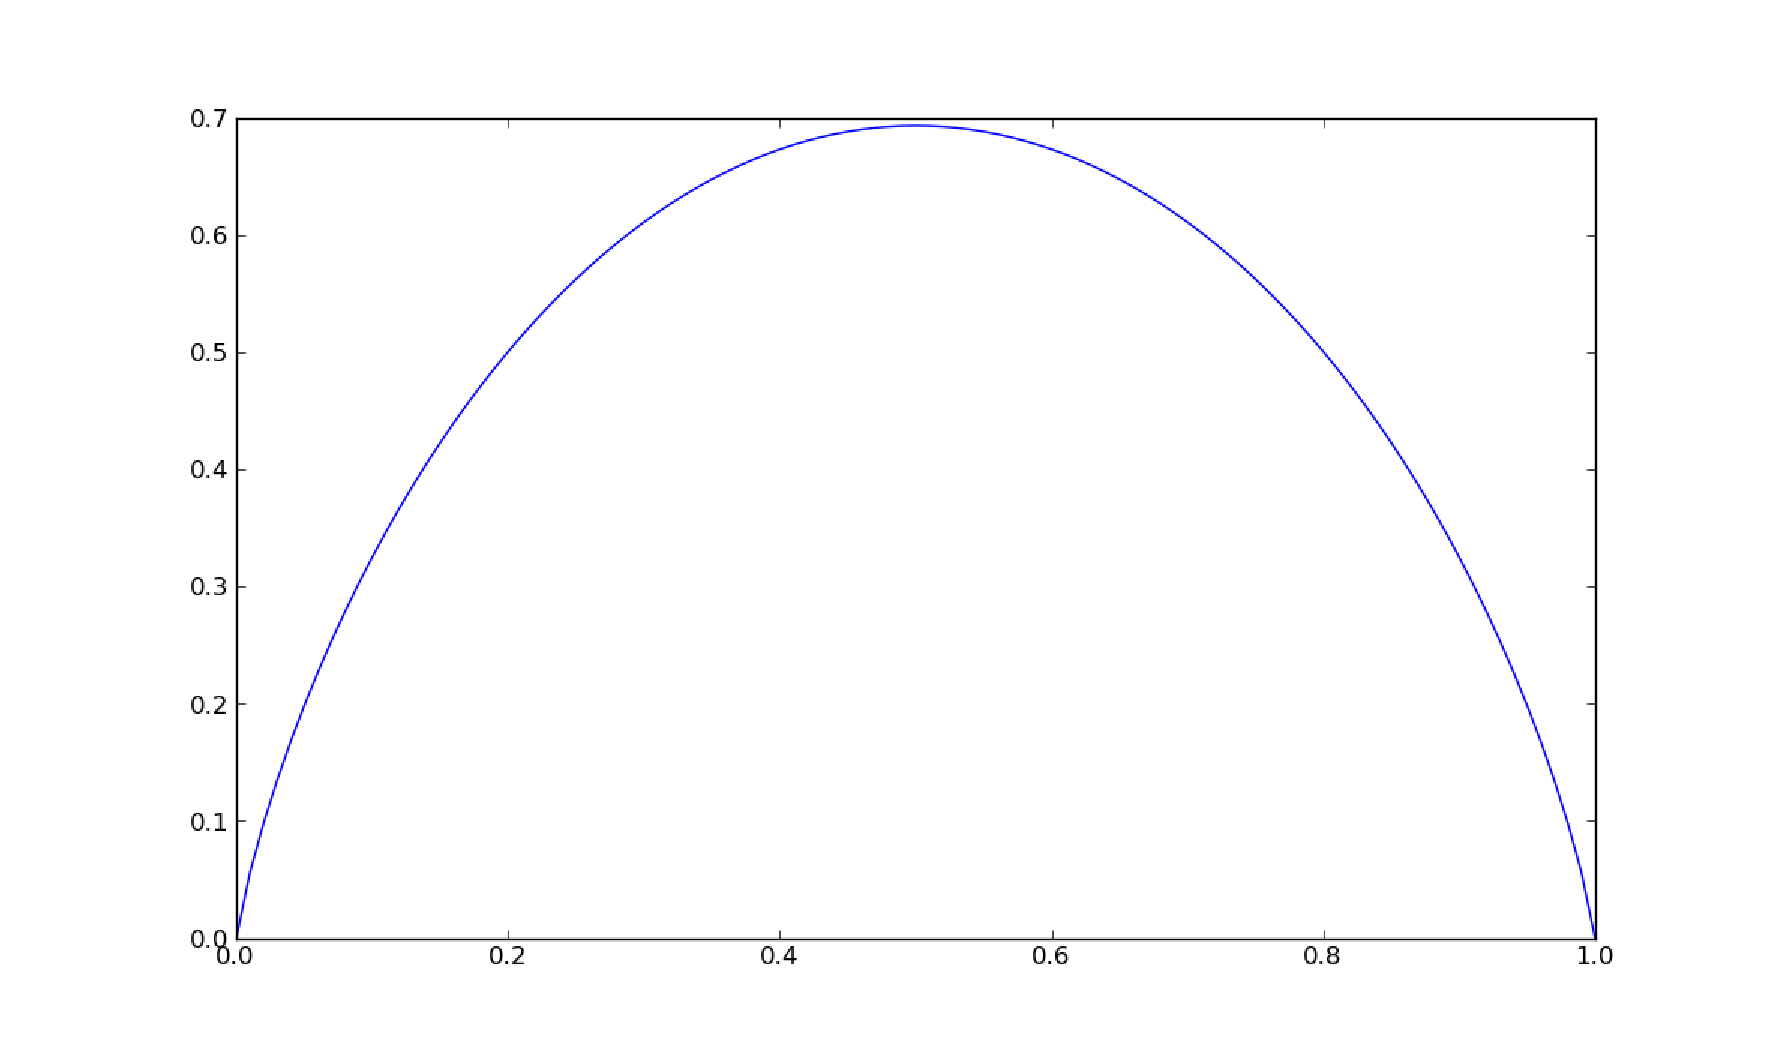
\includegraphics[width=\textwidth]{../images/entropy}
  \caption{The entropy function.}
  \label{class:entropy}
\end{figure}




Lets look at an example to see why this function could make sense. Suppose you are flipping a coin and would like to find a way to measure how biased it is. The probability that the coin flips tails is $p$ and heads is $1-p$. If your coin is highly biased and the probability of heads or tails is $1$ then $H(X)=0$, i.e. the random variable is always there same and has no information content or randomness. If the coin is fair, i.e. $P(X)=.5$ for both heads and tails, then $H(X)=1$, i.e. we have maximum randomness. 


From this example, there are a few intuitive conditions that one might come up with for such a function to exist: a) the function is symmetric and b) has a maximum at $.5$. There is actually one more technical condition which we won't get into here, but the three together ensure that the definition of $H(X)$ is unique up to a constant. If you are interested, in learning more about this I would recommend reading Claude Shannon's wonderful $1948$ paper \textit{A Mathemtical Theory of Communication} where in a tour de force of utter clarity and brilliance he laid out the foundation for information theory, signal processing, and really data science at large.


Back to decision trees\ldots Given a root node and a training set $T$

\begin{enumerate}
    \item calculate the entropy for each feature of your decision tree classifier 
    \item split $T$ into subsets using the feature for which entropy is minimum, i.e. for which we are reducing the randomness of our decision as much as possible
    \item make a decision tree node containing that feature, i.e. split
    \item continue on the above subsets with the remaining features
\end{enumerate}


Another way to say is that at each split we will maximize the \T{information gain} 

\begin{align*}
    IG(f) = H(T) - \sum_{s \in S} p(s)H(s)
\end{align*}

where $H(T)$ is the \T{entropy} of $T$, $S$ the subsets created by splitting $T$ over feature $f$, and $p(s)$ is the proportion of the number of elements in $s$ to the elements in $T$, i.e. the relative size of $s$. The above is known as the $ID3$ algorithm invented by Ross Quinlan. 



